\section{Auswertung}
	\label{sec:auswertung}
	
	Begonnen wurde mit Messaufgabe \ref{aufg:4}, da hierdurch schnell "uberpr"uft werden konnte, ob die Apparatur richtig justiert ist.
	Anschlie"send konnten alle anderen Messungen durchgef"uhrt werden.

	Die Schwierigkeit lag dabei in der Bestimmung der Winkel $\theta$, an denen die Intensit"at theoretisch sprunghaft, in der Realit"at jedoch stetig abnimmt.
	Hier wurde zun"achst die Intensit"at gegen die Energie aufgetragen, die sich nach 

	\begin{equation}
		E = \frac{\hbar c n}{2 d \sin{\theta}}
		\label{eqn:energie}
	\end{equation}

	berechnen lie"s (mit Lichtgeschwindigkeit $c$, Planck-Konstante $\hbar$, Gitterabstand $d$, Ord\-nung $n = 1$).

	Anschlie"send konnten wir dort die entsprechende Kante suchen.
	Wegen der Unsch"arfe der Messung wurde gem"a"s

	\begin{equation}
		E = \frac{1}{n} \sum_i^n E_i \nonumber
	\end{equation}

	ein Mittelwert "uber alle Energien $E_i$, die im Bereich der Kanten in Frage kommen gebildet.
	Abbildung \ref{fig:germanium} zeigt exemplarisch eine Messreihe f"ur ${}_{32}^{}\mathrm{Ge}$.
	Die einzelnen Mess\-pun\-kte werden miteinander verbunden, damit starke "Anderungen, die auf eine Kante hinweisen, besser zu erkennen sind.

	\begin{figure}[h!]
		\centering
		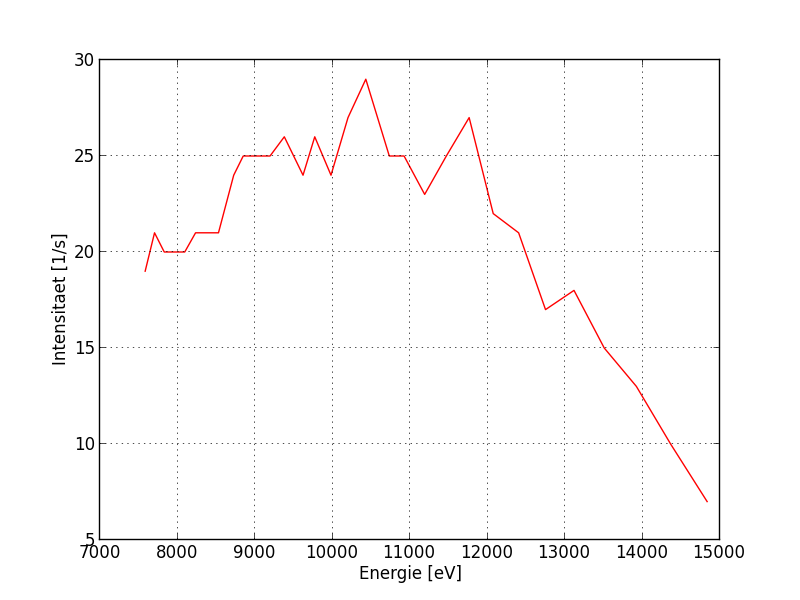
\includegraphics[width = 13cm]{img/graph_32_fein.png}
		\caption{Intensit"atsspektrum von Germanium}
		\label{fig:germanium}
	\end{figure}

	Durch die Messungenauigkeit $\Delta \theta = \SI{.1}{\degree}$ im Winkel erh"alt man mit Gau"s'scher Feh\-ler\-fort\-pflanz\-ung den Fehler

	\begin{equation}
		\Delta E = \left| \frac{\partial E}{\partial \theta} \right| \Delta \theta = 
		\frac{\hbar c}{2 d} \frac{\cos{\theta}}{\sin^2{\theta}} \Delta \theta . \nonumber
	\end{equation}

	\subsection{Energetisches Aufl"osungsverm"ogen}
		\label{subsec:aufloesung}

		Zun"achst wurde der LiF-Kristall auf einen Winkel $\theta = \SI{14}{\degree}$ eingestellt.
		Das Z"ahlrohr wurde vom Kristall entkoppelt und durchlief einen Winkelbereich von $\SI{26}{\degree}$ bis $\SI{30}{\degree}$.
		Das Intensit"atsmaximum lag bei $2\theta = \SI{28}{\degree}$, was auf eine richtig justierte Vorrichtung hin\-deu\-te\-te.

		\begin{figure}[h!]
			\centering
			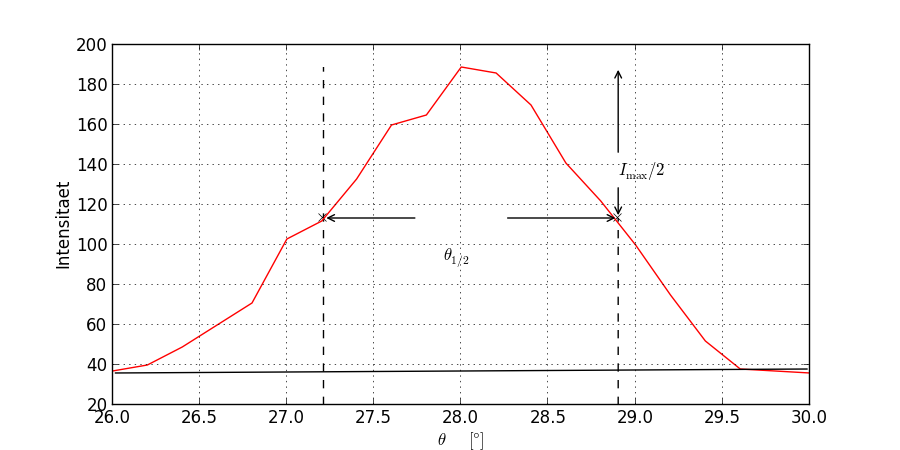
\includegraphics[width = 15cm]{img/graph_adjust.png}
			\caption{Messung zum Aufl"osungsverm"ogen}
			\label{fig:aufloesung}
		\end{figure}

		In der Abbildung \ref{fig:aufloesung} wurde die Winkelbreite $\theta_{1/2}$ der CuK-Emissionslinie markiert.
		Damit errechnen sich die Winkel zu $\theta_1 = \SI{27.2}{\degree}$ und $\theta_2 = \SI{28.9}{\degree}$ woraus sich mit \eqref{eqn:energie} die Energien $E_1 = \SI{6747.3}{\electronvolt}$ und $E_2 = \SI{6381.7}{\electronvolt}$ ergeben.

		Die Apparatur hat dann eine Aufl"osung von

		\begin{equation}
			\Delta E = E_1 - E_2 = \SI{365.6}{\electronvolt} \nonumber
		\end{equation}

		Eine Lineare Ausgleichsrechnung f"uhrt dann zu einem Winkel $\theta = \SI{5}{\degree}$ bei dem die Intensit"at verschwindet.
		Das entspricht einer Energie von $\SI{35.387}{\kilo \electronvolt}$. Der Wert weicht um $\SI{1.1}{\percent}$ vom erwarteten Wert ab. Die Kathodenspannung betrug $\SI{35}{\kilo \volt}$.

	\subsection{Abschirmzahlen $\sigma_{1,0}$ von ${}_{32}^{}\mathrm{Ge}$ und ${}_{41}^{}\mathrm{Nb}$}
		\label{subsec:abschirm1}
		Wie oben beschrieben wird die gemittelte Energie $E_\mathrm{K}$ bestimmt, an dem die K-Kanten von Germanium und Niob liegen. 
		Dadurch konnte mit 

		\begin{equation}
			\sigma_{1,0} = z - \sqrt{\frac{E_\mathrm{K}}{R_\infty} - \alpha^2 \frac{z^4}{4}} \nonumber
		\end{equation}

		die Abschirmungszahl $\sigma_{1,0}$ f"ur Elemente mit Kernladungszahl $z$ zwischen ungef"ahr 30 und 40 berechnet werden.
		Der Wert $R_\infty$ bezeichnet dabei die Rydberg-Energie, $\alpha$ die Sommerfeldsche Feinstrukturkonstante.

		Zudem ergibt sich mittels Gau"s`scher Fehlerfortplanzung ein weiterer Fehler

		\begin{equation}
			\Delta \sigma_{1,0} = \left| \frac{\partial \sigma_{1,0}}{\partial E_\mathrm{K}} \right| \Delta E_\mathrm{K} =
			\frac{1}{2 R_{\infty}} \sqrt{\frac{E_\mathrm{K}}{R_\infty} - \frac{1}{4} z^4 \alpha^2}^{-1}
			\cdot \Delta E_\mathrm{K} . \nonumber
		\end{equation}

		\begin{table}[h!]
			\centering
				\caption{Abschirmungszahlen f"ur Germanium und Niob. Die Energien wurden dabei direkt aus den entsprechenden Diagrammen entnommen.}
			\begin{tabular}{|c|c|c|}
				\hline
				Element & 
				$E_\mathrm{K}\,[\SI{}{\kilo \electronvolt}]$ & 
				$\sigma_{1,0}$ \\
				\hline \hline
				${}_{32}^{}\mathrm{Ge}$ & $\SI{10.581 (60)}{}$ & $\SI{4.11 (8)}{}$ \\
				${}_{41}^{}\mathrm{Nb}$ & $\SI{18.461 (188)}{}$ & $\SI{4.16 (18)}{}$ \\
				\hline
			\end{tabular}
		\end{table}

	\subsection{Abschirmzahlen $s_{2,1}$ von ${}_{79}^{}\mathrm{Au}$ und ${}_{80}^{}\mathrm{Hg}$}
		\label{subsec:abschirm2}
		F"ur Elemente mit Kernladungszahl $z$ zwischen 73 und 83 lie"s sich die Abschirmungszahl $s_{2,1}$ wurden die $L_\mathrm{III}$- und $L_\mathrm{II}$-Kanten ermittelt.
		Grund hierf"ur ist die geringe Aufl"osung des Apparates, die es nicht erm"oglicht, eine $L_\mathrm{I}$-Kante zu identifizieren.
		$E_\mathrm{L}$ bezeichnet im Folgenden die Differenz $E_\mathrm{L_\mathrm{III}} - E_\mathrm{L_\mathrm{II}}$.
		
		N"aherungsweise gilt dann

		\begin{equation}
			s_{2,1} = z - \left[\left( \frac{4}{\alpha} \sqrt{\frac{E_\mathrm{L}}{R_\infty}} - \frac{5 E_\mathrm{L}}{R_\infty} \right)
			\left( 1 + \frac{19}{32}\alpha^2 \frac{E_\mathrm{L}}{R_\infty} \right)\right]^{1/2} . \nonumber
		\end{equation}

		Auch diese Gr"o"se ist fehlerbehaftet. Gau"s'sche Fehlerfortpflanzung liefert

		\begin{eqnarray*}
			\Delta s_{2,1} & = & \left|\frac{\partial s_{2,1}}{\partial E_\mathrm{L}}\right| \cdot \Delta E_\mathrm{L} \quad = \\
			& = & \frac{-95 \alpha^3 E_\mathrm{L}^{3/2} + 57 \alpha^2 E_\mathrm{L} \sqrt{R_\infty} - 80\alpha R_\infty \sqrt{E_\mathrm{L}} + 32 R_\infty^{3/2}}{4 \alpha R_\infty^2 \sqrt{2 E_\mathrm{L} \left( \frac{4E_\mathrm{L}^{1/2}}{\alpha R_\infty^{1/2}} - \frac{5E_\mathrm{L}}{R_\infty} \right) \left( \frac{19 \alpha^2 E_\mathrm{L}}{R_\infty} + 32 \right)}} \cdot \Delta E_\mathrm{L}.
		\end{eqnarray*}

		Wir erhalten:

		\begin{table}[h!]
			\centering
			\begin{tabular}{|c|c|c|c|c|}
				\hline
				Element & 
				$E_\mathrm{L_\mathrm{III}}\,[\SI{}{\kilo \electronvolt}]$ &
				$E_\mathrm{L_\mathrm{II}}\,[\SI{}{\kilo \electronvolt}]$ &
				$E_\mathrm{L}\,[\SI{}{\kilo \electronvolt}]$ & 
				$s_{2,1}$ \\
				\hline \hline
				${}_{79}^{}\mathrm{Au}$ & 
					$\SI{8.812 (41)}{}$ &
					$\SI{7.964 (33)}{}$ & 
					$\SI{.848 (74)}{}$ & 
					$\SI{15.64 (14)}{}$ \\
				${}_{80}^{}\mathrm{Hg}$ & 
					$\SI{8.773 (40)}{}$ &
					$\SI{7.964 (33)}{}$ &
					$\SI{.808 (73)}{}$ & 
					$\SI{17.34 (15)}{}$ \\
				\hline
			\end{tabular}
		\end{table}

	\subsection{Abschirmzahlen $\sigma_1$ und $\sigma_2$ f"ur ${}_{29}^{}\mathrm{Cu}$}
		\label{subsec:kupfer}
		Wir suchen nun die Energien f"ur die $K_\alpha$-- und $K_\beta$--Kanten im Emissionsspektrum von Kupfer, weil wir daraus $\sigma_1$ und $\sigma_2$ bestimmen k"onnen.
		Nach der Ermittlung dieser Werte liefert die Anleitung folgende N"aherungen:

		\begin{eqnarray}
			\sigma_1 & = & z - \sqrt{\frac{E_\mathrm{K_\beta}}{R_\infty}} , \nonumber \\ 
			\sigma_2 & = & z - \sqrt{4\left(\left( z - \sigma_1 \right)^2 - \frac{E_\mathrm{K_\alpha}}{R_\infty} \right)} . \nonumber
		\end{eqnarray}

		Die Messung liefert uns folgende Ergebnisse:

		\begin{eqnarray}
			E_\mathrm{K_\alpha} & = & \SI{7.964 (33)}{\kilo \electronvolt} \nonumber \\
			E_\mathrm{K_\beta} & = & \SI{8.773 (41)}{\kilo \electronvolt} \nonumber \\
			\Rightarrow \qquad \sigma_1 & = & \SI{3.61 (4)}{} \nonumber \\
			\Rightarrow \qquad \sigma_2 & = & \SI{13.63 (50)}{} . \nonumber
		\end{eqnarray}

		Auch hier wurde die Gau"s'sche Fehlerfortpflanzung beachtet.